\documentclass[aip,amsmath,amssymb,reprint,floatfix]{revtex4-1}

\usepackage[utf8]{inputenc}
\usepackage[T1]{fontenc}
\usepackage{mathptmx}
\usepackage{etoolbox}
\usepackage{graphicx}
\usepackage{dcolumn}
\usepackage{bm}
\usepackage{subcaption}
\usepackage{lipsum}
\usepackage{amsmath,amssymb}
\usepackage{placeins}

\makeatletter
\def\@email#1#2{
 \endgroup
 \patchcmd{\titleblock@produce}
  {\frontmatter@RRAPformat}
  {\frontmatter@RRAPformat{\produce@RRAP{*#1\href{mailto:#2}{#2}}}\frontmatter@RRAPformat}
  {}{}
}
\makeatother
\begin{document}


\title[Moderator Simulation for the Compact Positron Source at NLCTA]{Moderator Simulation for the Compact Positron Source at NLCTA}
\author{Ryland Goldman}
\email{rgoldman@slac.stanford.edu}
\affiliation{SLAC National Accelerator Laboratory, Menlo Park, California 94025, USA}
\affiliation{Department of Physics and Astronomy, University of California, Los Angeles, Los Angeles, California 90095, USA}

\author{Sophie Crisp}
\affiliation{SLAC National Accelerator Laboratory, Menlo Park, California 94025, USA}

\author{Spencer Gessner}
\affiliation{SLAC National Accelerator Laboratory, Menlo Park, California 94025, USA}

\date{\today}

\begin{abstract}
Positron moderation is a key part in the production of slow positrons. This paper examines G4beamline simulations of various moderator designs and the addition of a radiofrequency cavity to increase the efficiency of the moderator. A setup consisting of a 100~MeV electron beam incident on a 7~mm tungsten target, a 5~T adiabatic matching device, a 5-cell L-band RF cavity, and a single-crystal tungsten moderator leads to a 39.3x improvement in the number of positrons moderated over a common thin-foil polycrystalline moderator without the AMD and cavity. We also present a novel calculation method for determining the stopping distribution of low-energy positrons in a thin foil, modifying the Makhovian distribution with an exponential ramp to account for edge effects.
\end{abstract}

\maketitle

\section{Introduction}
Slow positrons are positrons with kinetic energy on the order of single eV. Among other fields, these positrons have applications in positron annihilation spectroscopy, ultrafast positron diffraction, and antimatter research. The Next Linear Collider Test Accelerator (NLCTA) at SLAC is currently in the planning stage for a compact positron source which produces slow positrons from an electron linac.

A target (also referred to as a ``converter'' by some sources) produces an electromagnetic shower when the high-energy electrons interact with high-Z nuclei through Coulomb scattering. The resulting Bremsstrahlung radiation is capable of producing electron-positron pairs. These positrons are collimated by an adiabatic matching device and then decelerated using a radiofrequency cavity.

We then capture these positrons by stopping them inside of a tungsten moderator, where the negative work function of the material causes some to be reemitted from the surface at KE=2.8 eV.~\cite{Wilson} This project attempts to optimize the positron yield from a target-moderator system using G4beamline, a particle tracking program derived from the GEANT4 toolkit.~\cite{G4beamline,GEANT4} The Penelope2008 models~\cite{Salvat2009} are used via the FTFP\_BERT\_PEN physics package. Most simulations were parallelized to run on a 192-core c6a.metal instance on AWS EC2.

\section{Target}
Initially, the target parameters (thickness and composition) are selected to optimize the positron yield $\gamma_t$, defined as the fraction of positrons emitted from the target to the number of electrons in. We simulate a 100 MeV electron beam directly incident on a target of varying thickness. The number of positrons produced in the forward direction is divided by the number of incident electrons as shown in Fig.~\ref{fig:yield_vs_thickness}, which agrees with the data found by previous groups.~\cite{ORourke}

The optimal thickness is found to be 6.5~mm for tungsten and 7.0~mm for tantalum, and the yield at optimal thickness to be $0.2330\pm0.0013$ positrons per incident electron for tungsten compared to $0.2318\pm 0.0013$ for tantalum.

\begin{figure}
    \centering
    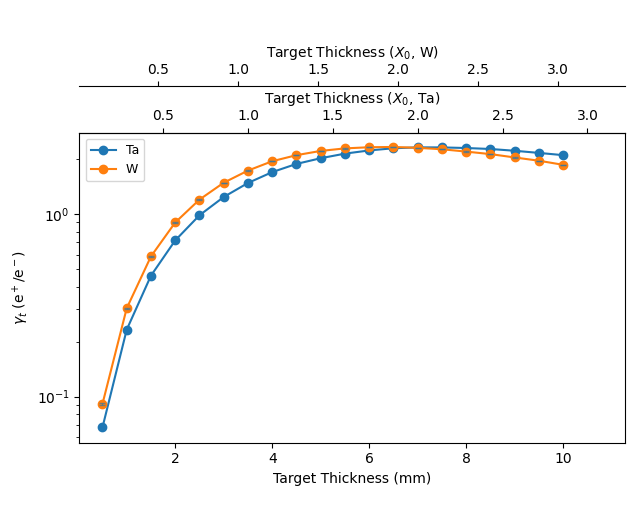
\includegraphics[width=\linewidth]{yield_v_thickness.png}
    \caption{Positron yield $\gamma_t$ as a function of target thickness (shown in both millimeters and radiation lengths) for tungsten and tantalum. We use 100 MeV electrons; see~\cite{ORourke}~for a comparable plot with different electron energies.}
    \label{fig:yield_vs_thickness}
\end{figure}

As there is no significant performance difference for determining the target material, we instead consider the material properties. Due to its melting point, the GBAR project at CERN chose to use tungsten to prevent ablation by the electron beam.~\cite{GBAR, Liszkay} Tungsten is also significantly less expensive than tantalum.~\cite{Liszkay}

Therefore, we select a tungsten target with a thickness of 7.0~mm, which is used for the remainder of this paper. Fig.~\ref{fig:energytarget} shows the energy spread of the resulting positrons, which peaks at approximately 3 MeV.

\begin{figure}
    \centering
    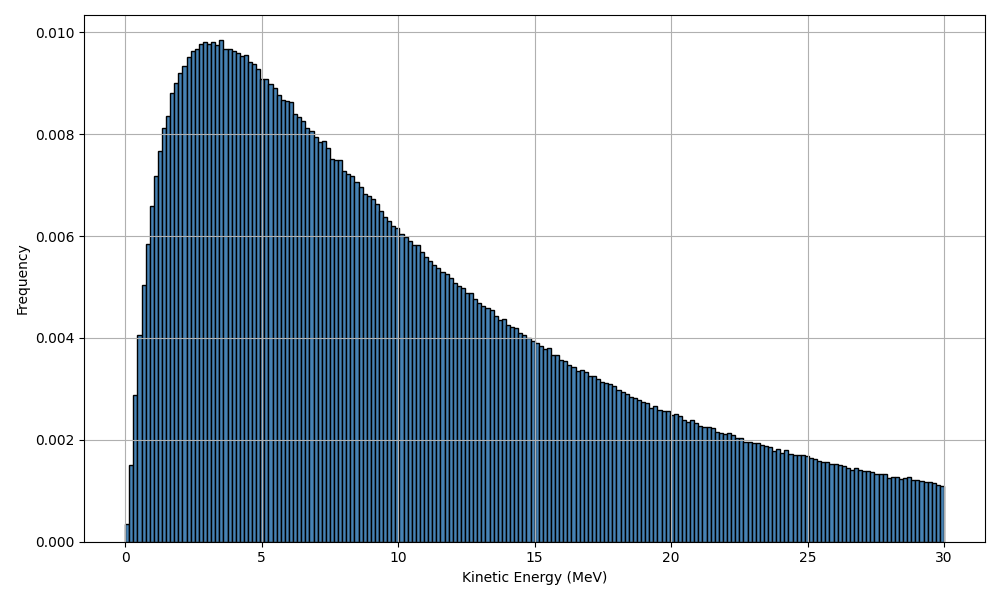
\includegraphics[width=\linewidth]{energy_target_out.png}
    \caption{Energy distribution histogram of positrons emitted in the forward direction from 100 MeV electron collisions with a~7.0~mm tungsten target.}
    \label{fig:energytarget}
\end{figure}


\section{Adiabatic Matching Device}
The positrons emitted from the target have a wide angular divergence which must be reduced in order for the beam to pass through the RF cavity. We use an adiabatic matching device (AMD), which consists of a solenoidal magnetic field decreasing from 5.0~T to 0.5~T with the formula,
\begin{eqnarray}
    B_z(\rho=0)=\frac{B_0}{1+\alpha z}\\
    B_\rho(\rho,z)=\frac{B_0\alpha\rho}{2\left( 1+\alpha z \right)^2},
\end{eqnarray}
where $\alpha=0.018$~mm$^{-1}$ is the tapering parameter.~\cite{AMD,AMDslac}

\begin{figure}
    \centering
    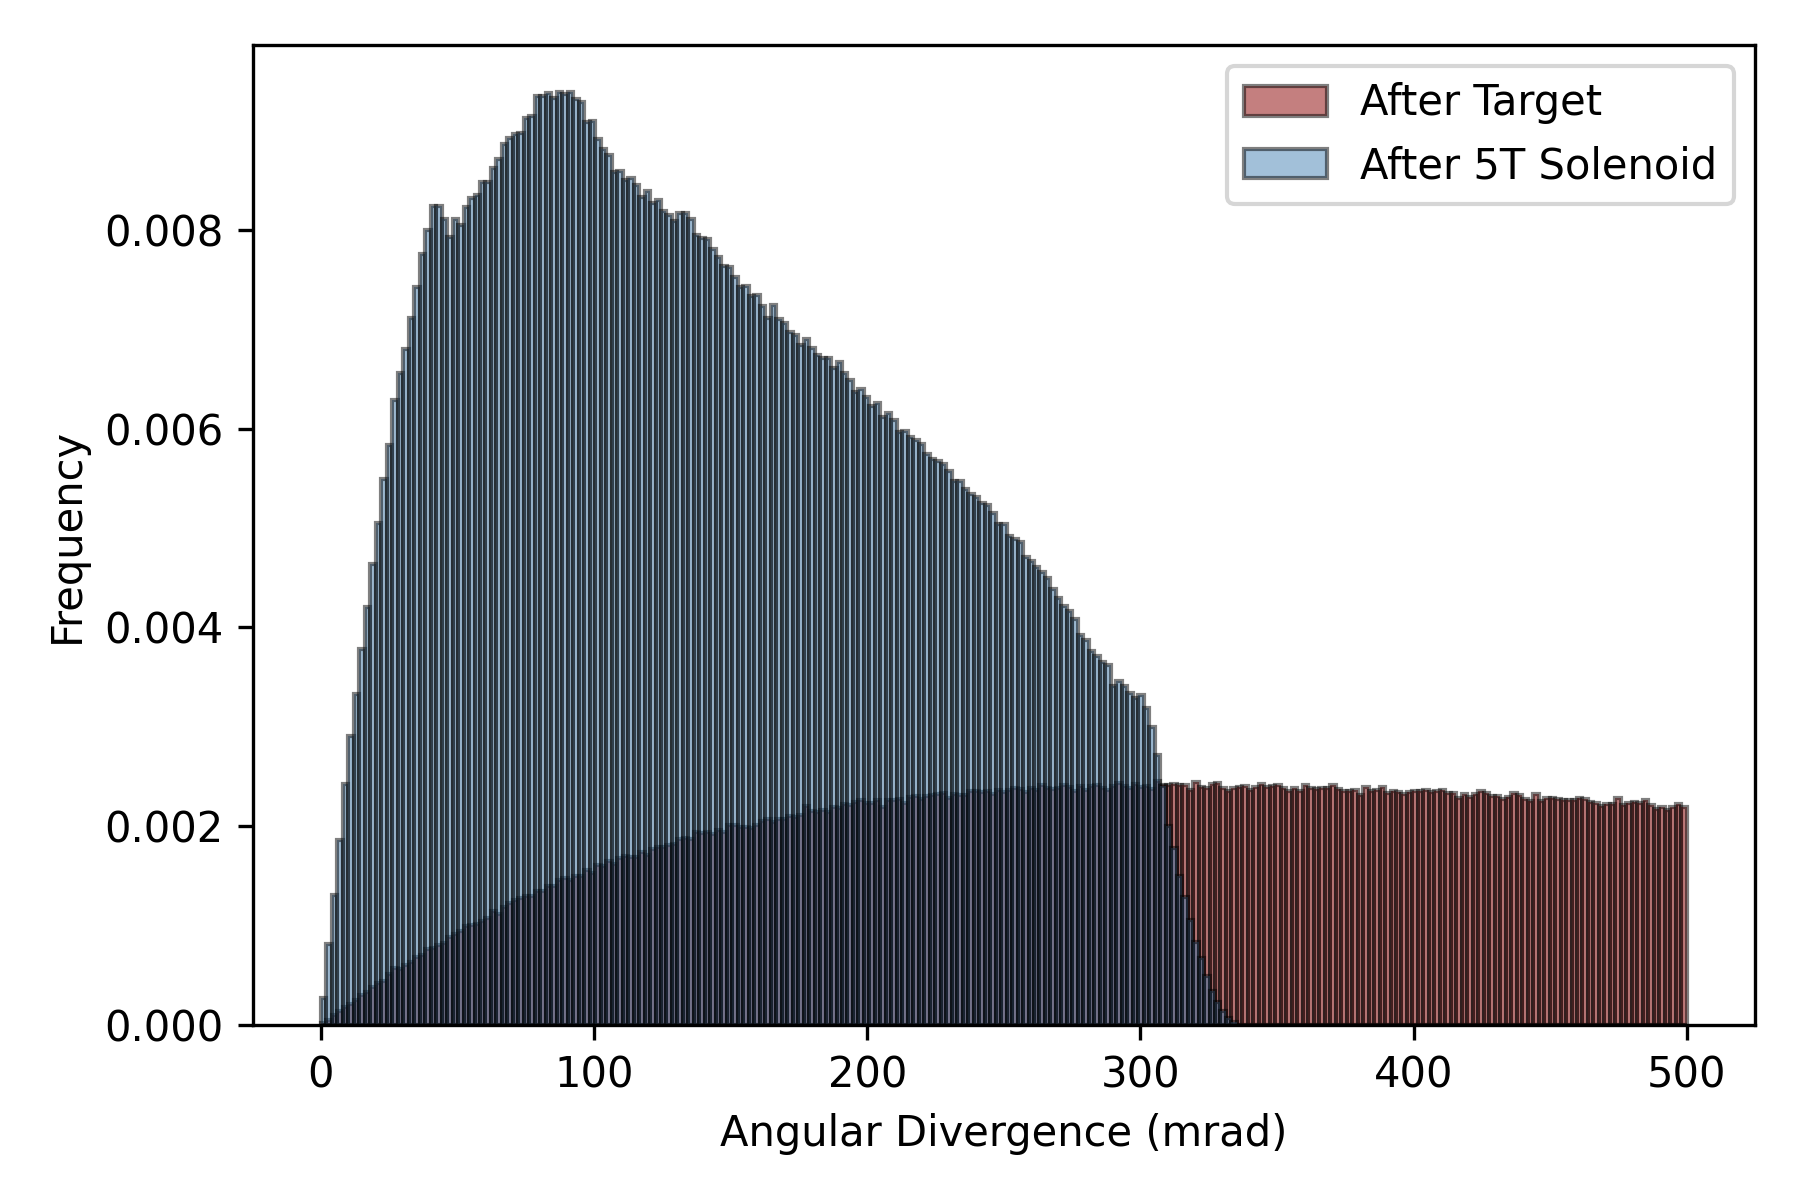
\includegraphics[width=\linewidth]{AMDOut.png}
    \caption{Angular divergence histogram of positrons before and after passing through the adiabatic matching device. The AMD reduces the spread of nearly all particles to under 300 mrad.}
    \label{fig:AMD}
\end{figure}
\begin{figure}
    \centering
    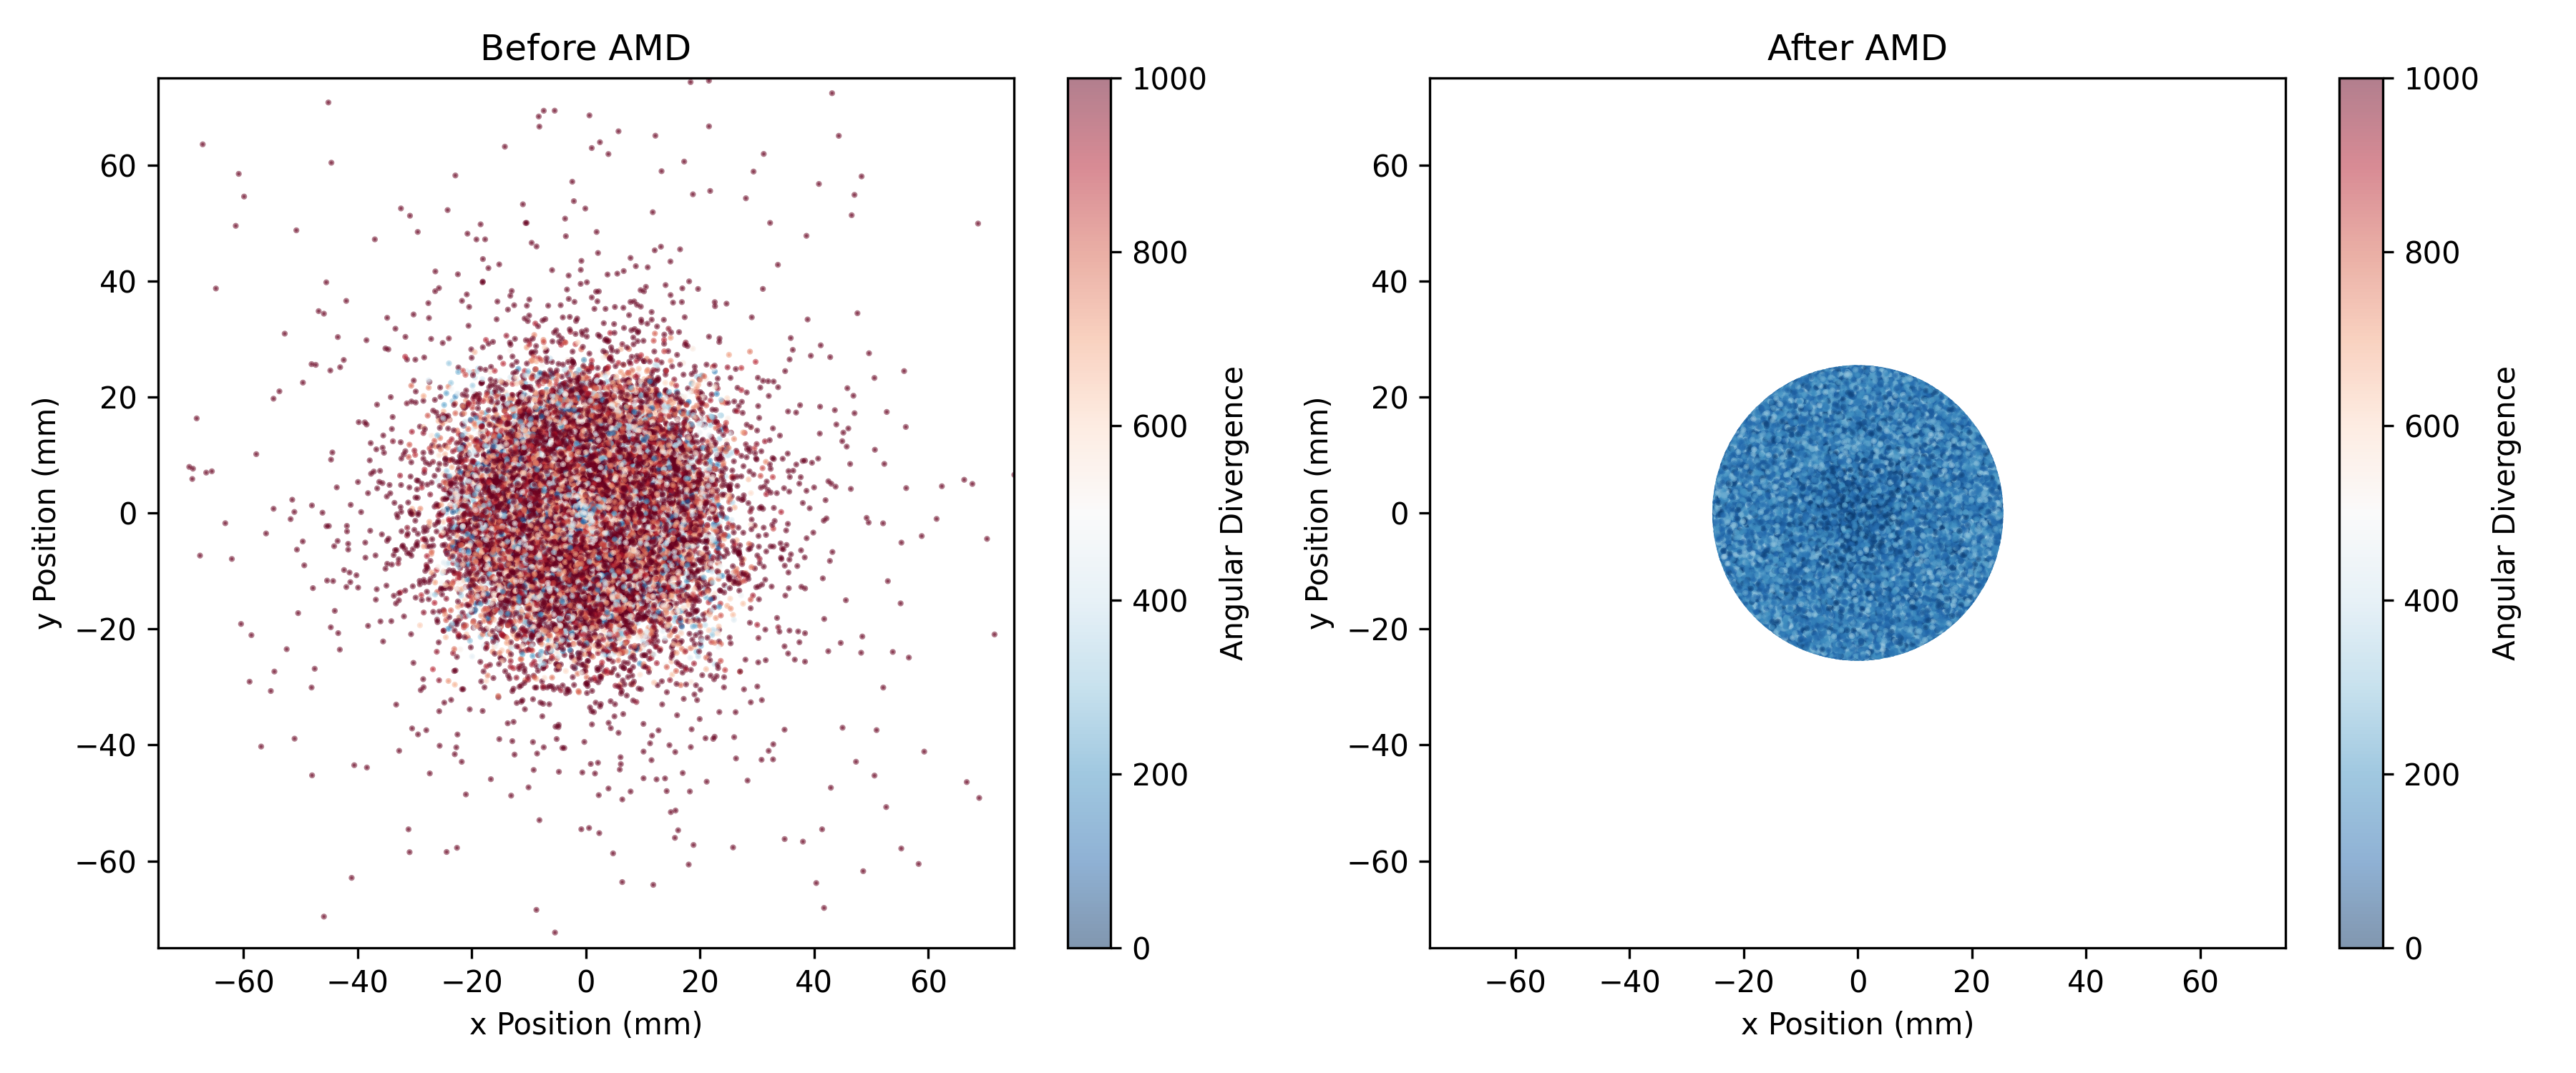
\includegraphics[width=\linewidth]{AMDOut2.png}
    \caption{Cross-section of positron beam a) emitted by the target, and b) after leaving the AMD, colored by angular divergence. The AMD was modeled as a 25mm cylinder.}
    \label{fig:AMD2}
\end{figure}

As shown in Fig.~\ref{fig:AMD}, the AMD reduces the beam's angular divergence to within acceptable levels. Fig.~\ref{fig:AMD2} additionally shows the beam's transverse displacement. Particles with $r>25$ mm are removed from the simulation as they are assumed to come in contact with the edge of the AMD.

Of the high-energy positrons emitted from the target, 69.9\% survive the AMD and pass into the RF cavity.

\section{Moderator Theory}
\subsection{Makhovian Distribution}
The stopping distribution of positrons in a thick material is described by the Makhovian distribution,
\begin{equation}
    p(z)=\frac{m\,z^{m-1}}{(z_0)^m}\exp\left( \left( -\frac{z}{z_0} \right)^m \right),
\end{equation}
where $p(z)$ is a probability density function and $m$ and $z_0$ are constants determined by the positron's angle of incidence and energy~\cite{Alsulami}. For normal incidence, $m=1.89$, with the values for $z_0$ as listed in Table~\ref{tab:makhov}.

\begin{table}[h]
\centering
\caption{Makhovian distribution parameter $z_0$ for tungsten for varying positron kinetic energies (KE) at normal incidence. There is variation between physics packages and these constants may not perfectly match those from other simulation software packages.~\cite{DRYZEK20084000}}
\label{tab:makhov}
\begin{ruledtabular}
\begin{tabular}{cccc}
&KE (MeV) & $z_0$ (µm) \\
\hline
&0.1 & $3.85\pm0.045$ & \\
&0.5 & $43.50\pm0.19$ & \\
&1.0 & $105.54\pm0.27$ &  \\
&5.0 & $649.72\pm 1.13$ & \\
&10.0& $1349.36\pm1.78$ \\
\end{tabular}
\end{ruledtabular}
\end{table}


\subsection{Optimization}
Sample values for the Makhovian distribution at different energies are shown in Fig.~\ref{fig:Makhovian}. For a beam with a wide energy spread, only the low-energy particles are stopped in the moderator (Fig.~\ref{fig:FoilEnergy}). 27.2\% of positrons with kinetic energies under 500 keV stop. Additionally, many of these low-energy positrons are reflected off of the moderator surface.

To ensure that the greatest quantity of positrons stop in the moderator, the energy of the beam must be reduced using a decelerating cavity (see Section V).

\begin{figure}
    \centering
    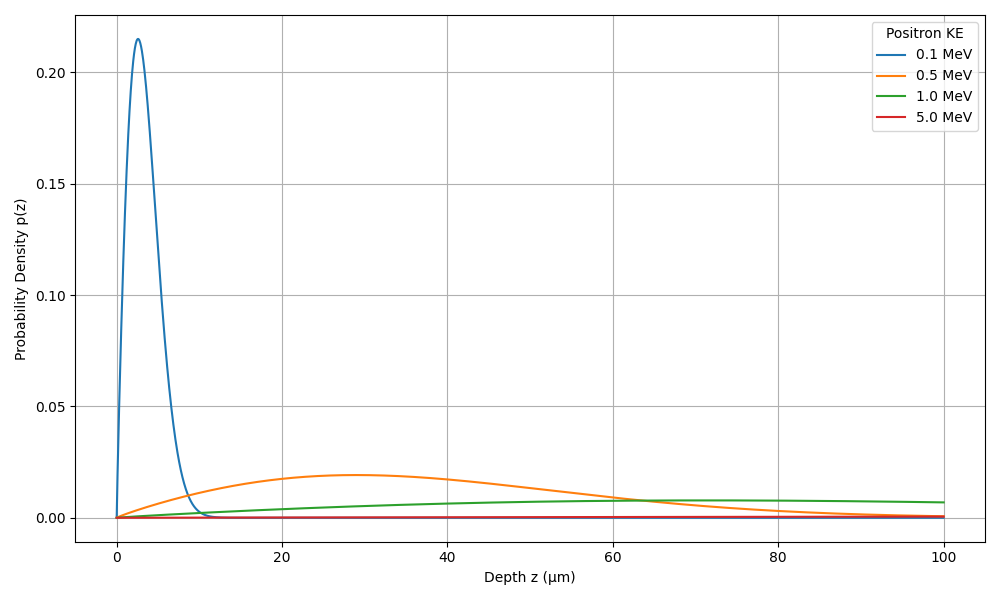
\includegraphics[width=\linewidth]{Makhovian.png}
    \caption{Makhovian distributions at normal incidence for different positron energies. As expected, lower energy positrons stop much sooner.}
    \label{fig:Makhovian}
\end{figure}

\begin{figure}
    \centering
    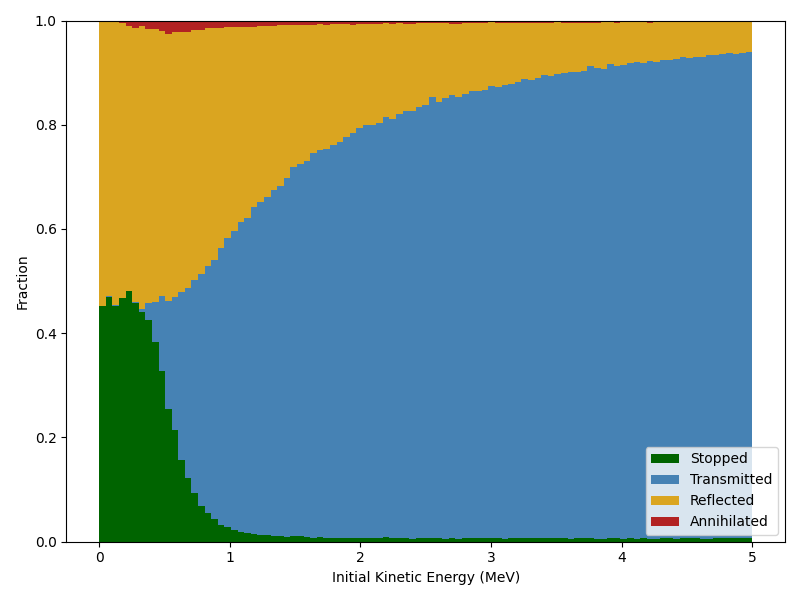
\includegraphics[width=\linewidth]{50_energy_fraction.png}
    \caption{Outcome of incoming positrons in a 50 µm foil moderator, categorized by initial kinetic energy. Positrons with energy over 1 MeV essentially do not contribute to the moderator yield.}
    \label{fig:FoilEnergy}
\end{figure}


\subsection{Ramped Makhovian}
In a thin foil, the positrons do not follow the Makhovian distribution exactly. As an example, Fig.~\ref{fig:BackscatteringExample} shows the trace of a particle with 900 keV kinetic energy. This particle would eventually come to rest at 38 µm (blue line) and contributes to the Makhovian distribution at that point. However, in a 50 µm foil (red line), it would escape before it could scatter backwards and stop.

\begin{figure}
    \centering
    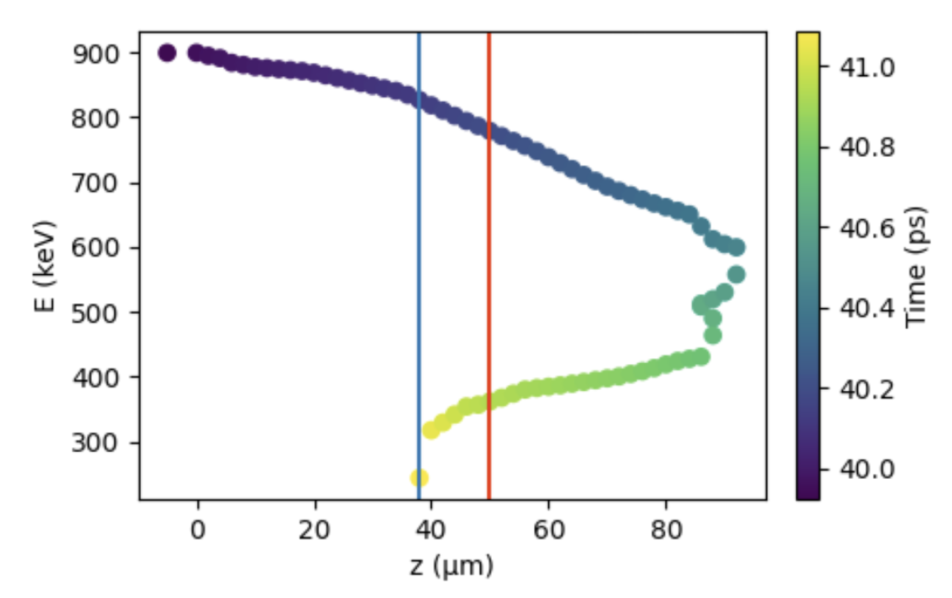
\includegraphics[width=\linewidth]{BackscatteringExample.png}
    \caption{Particle trace of an incident positron that would contribute to the Makhovian, but passes through a thin foil. The blue line indicates the final stopping point of the particle in a semi-infinite material, while the red line indicates the border of a 50 µm moderator.}
    \label{fig:BackscatteringExample}
\end{figure}

If the probability of a particle escaping increases exponentially to 100\% at the border, the Makhovian distribution should be attenuated by an exponential ramp
\begin{equation}
    \tilde{p}(z)=p(z)\left( 1-\exp\left( -\frac{L-z}{\lambda} \right) \right),
\end{equation}
where $L$ is the moderator length and $\lambda$ is a constant dependent on $L$. This function is a good approximation of the distribution for thin foils, as shown in Fig.~\ref{fig:RampedMakhovian}. The fit parameters for Fig.~\ref{fig:RampedMakhovian} are listed in Table~\ref{tab:RampedMakhovian}.

\begin{figure}
    \centering
    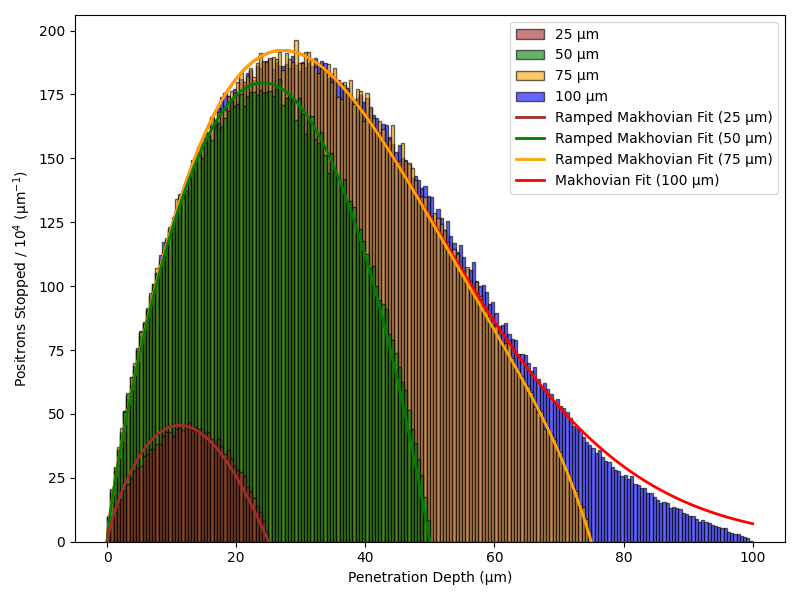
\includegraphics[width=\linewidth]{RampedMakhovian.png}
    \caption{Simulation (shaded) and ramped Makhovian fits for 500 keV positrons on foils of various thicknesses. The red line is an unramped Makhovian for the 100 µm foil.}
    \label{fig:RampedMakhovian}
\end{figure}
\begin{table}[h]
\centering
\caption{Ramped Makhovian distribution parameter $\lambda$ for 500 keV positrons on a thin tungsten foil}
\label{tab:RampedMakhovian}
\begin{ruledtabular}
\begin{tabular}{cccc}
&Foil Thickness (µm) & $\lambda$ (µm) \\
\hline
&25 & $32.94\pm0.42$ & \\
&50 & $9.00\pm0.12$ & \\
&75 & $4.65\pm0.21$ &  \\
\end{tabular}
\end{ruledtabular}
\end{table}


\section{L-Band Cavity}
To decelerate the beam, we use a five-cell $L$-band (1.3 GHz) radiofrequency cavity previously developed for the ILC linac~\cite{PhysRevSTAB.12.042001}. The cavity has been tested up to a gradient of 13.7 MV/m, but we simulate it at a higher gradient of 15 MV/m.

The search method used to locate the optimal timing offsets for each cell was a Monte Carlo simulated annealing algorithm. Several random initial conditions are chosen throughout parameter space. Similar to a gradient descent, neighboring points are evaluated for the cost function (for example, maximizing particles under 200 keV), but less optimal solutions are accepted probabilistically to escape any local minima. The step size and acceptance probability (temperature) are decreased over time to mimic the annealing of materials. This method is preferable to a gradient descent as it requires less compute time.

\begin{figure}
    \centering
    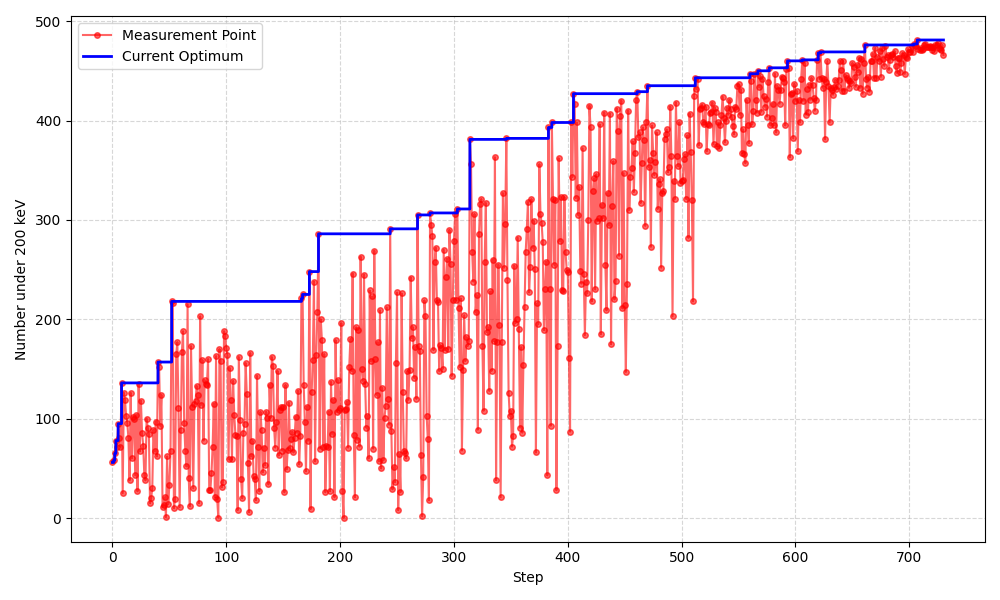
\includegraphics[width=\linewidth]{SimulatedAnnealing.png}
    \caption{The simulated annealing algorithm used to tune RF cavity. Here, the goal was to optimize the number of positrons under 200 keV, which are the most likely to stop in the moderator. Different goals were used to produce the greatest yield in each moderator.}
    \label{fig:SimulatedAnnealing}
\end{figure}

\begin{figure}
    \centering
    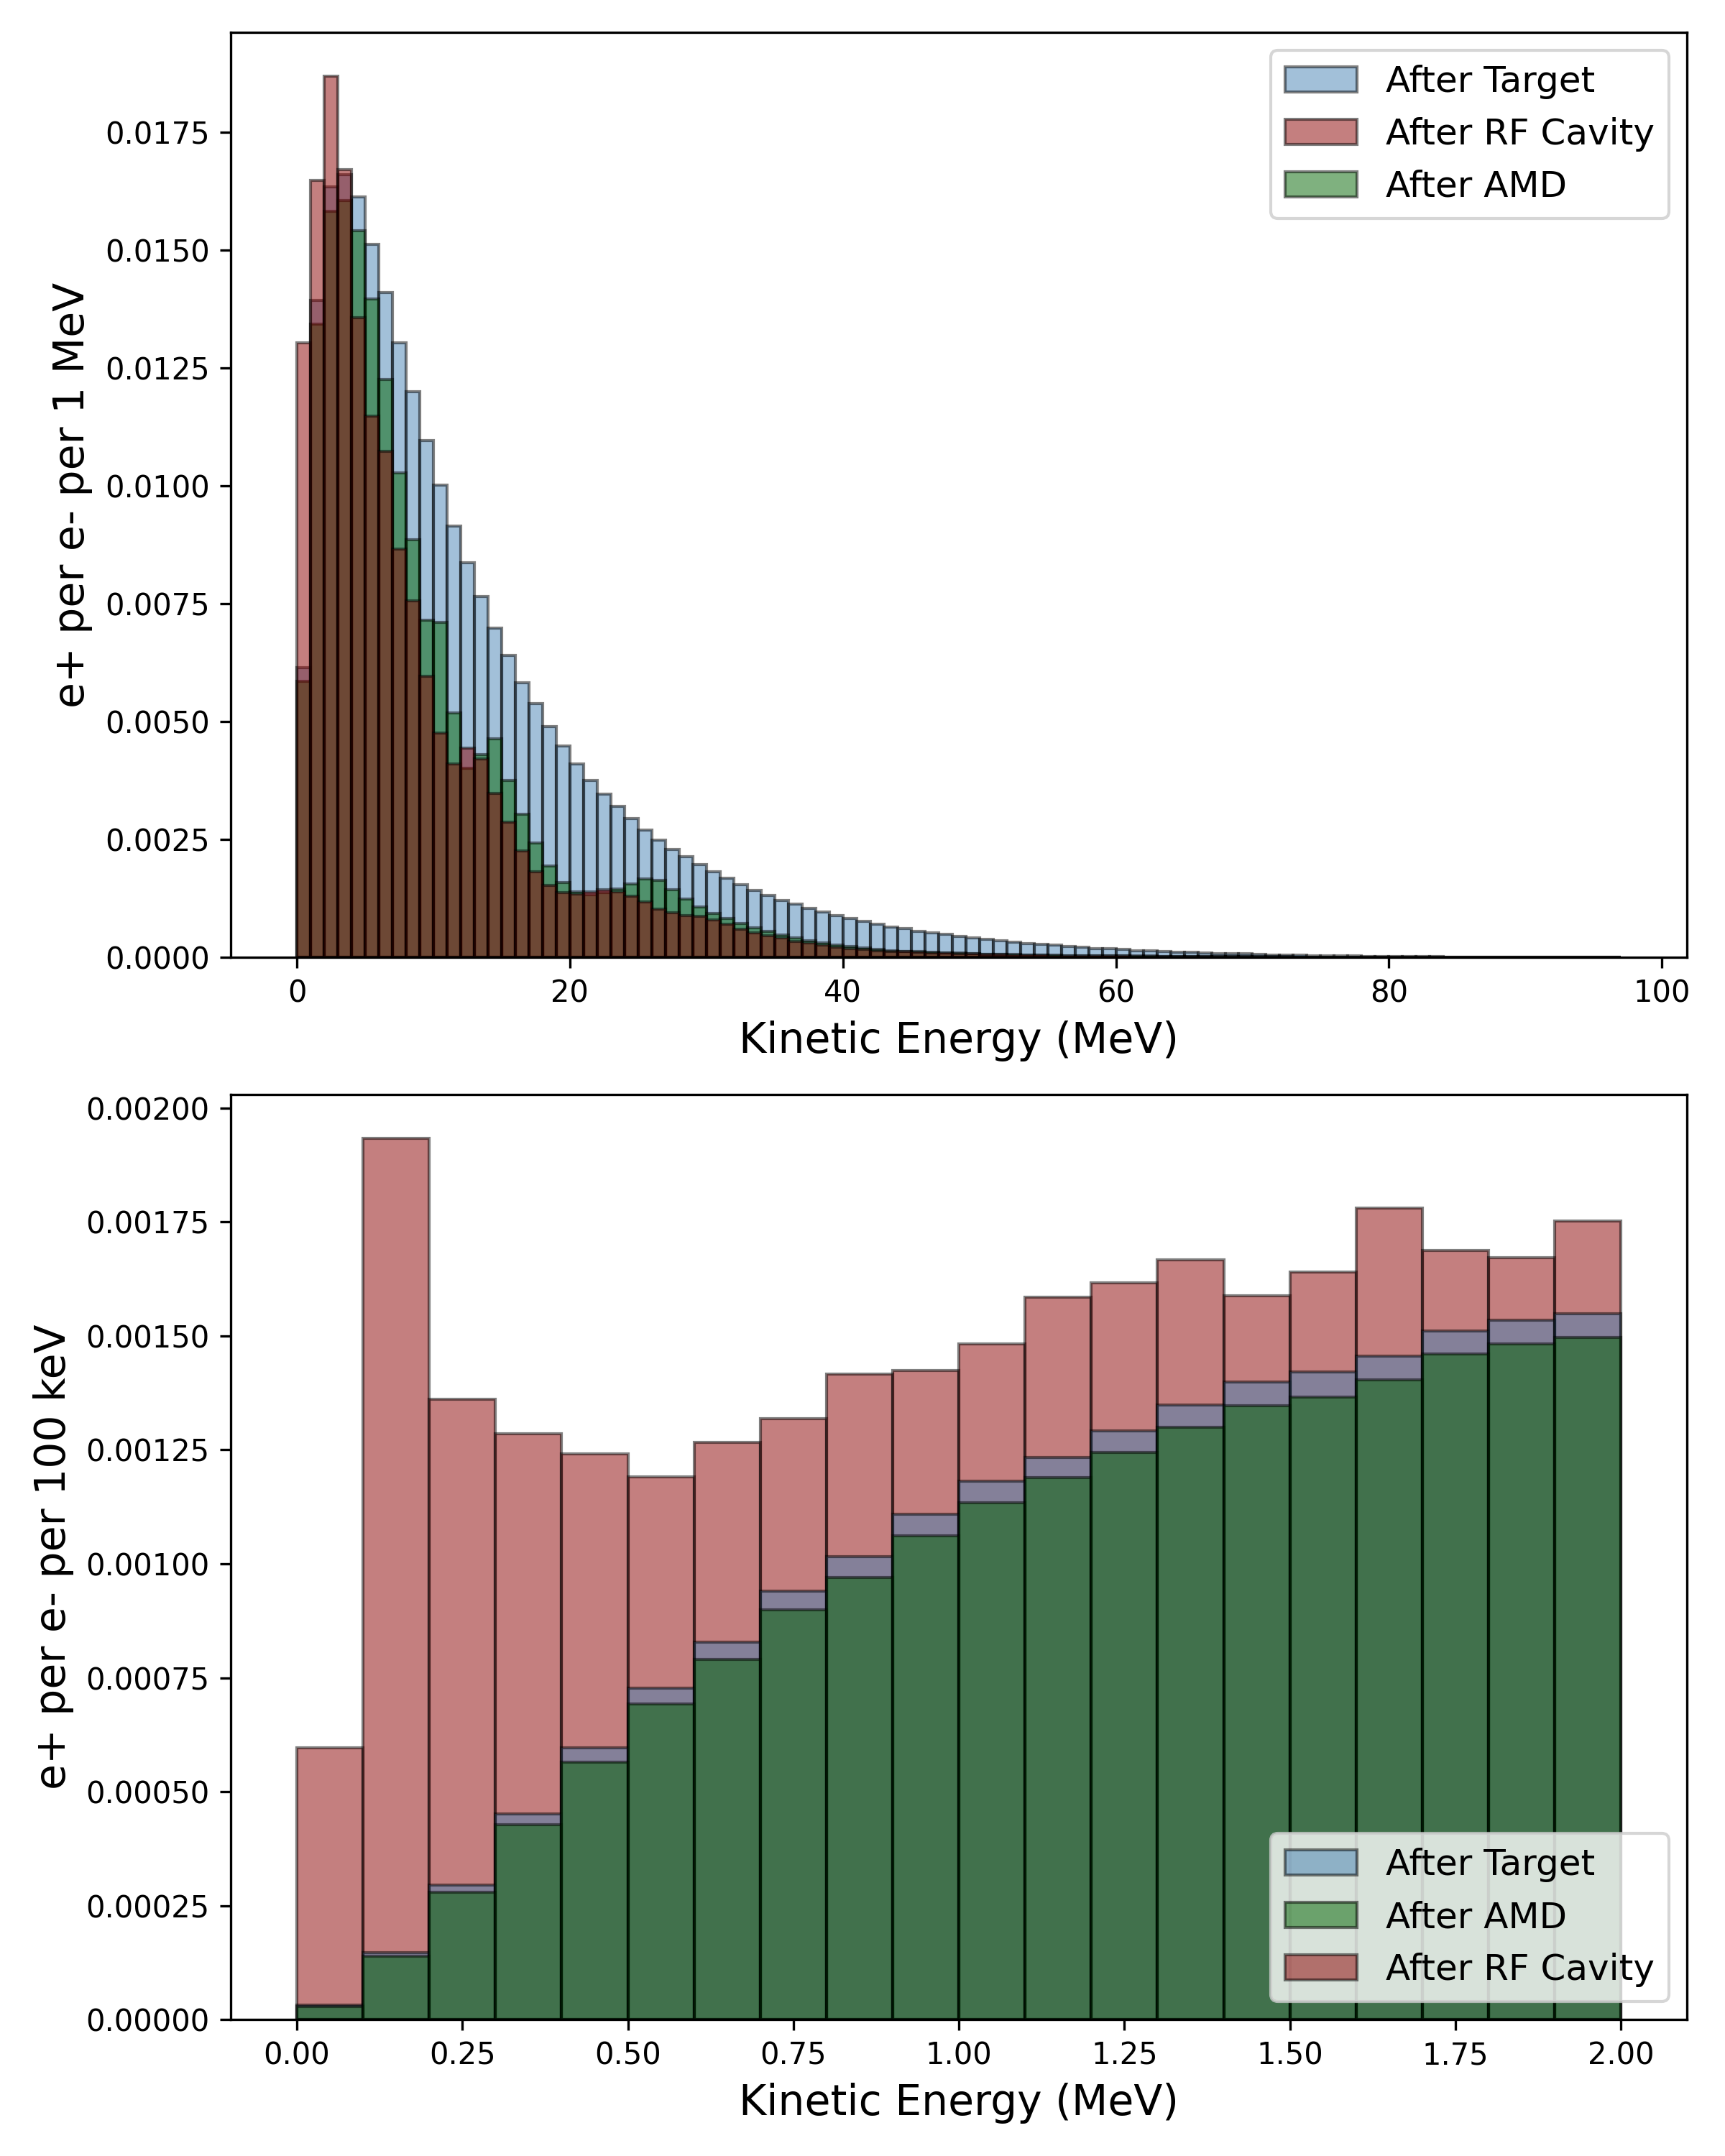
\includegraphics[width=\linewidth]{LBandOut.png}
    \caption{Resulting energy distribution of positrons before and after passing through the RF cavity. The distribution has been shifted towards lower energies.}
    \label{fig:LBand}
\end{figure}

Fig.~\ref{fig:LBand} shows the result of this optimization. The cavity improved the number of positrons with $KE<200$~keV by a factor of 15.


\section{Positron Thermalization}
Due to the negative work function of tungsten, the positrons that stop close to the surface of the foil can be ejected from the moderator~\cite{Wilson}. The number of ejected positrons is characterized by a diffusion length $L_+$. For polycrystalline tungsten, $L_+=55$ nm. For single-crystal tungsten, $L_+=135$ nm.

The probability of thermalization for a particle is given by
\begin{equation}
    P_\text{thermalization}(z)=\exp\left( -\frac{z}{L_+} \right),
\end{equation}
with $z$ representing the distance to the surface~\cite{ORourke}.

This can also be written as an integral over the stopping distribution $\tilde{p}(z)$,
\begin{equation}
    \label{eq:therm}
    P_\text{thermalization}=\int_0^L \tilde{p}(z)\left[ e^{-\frac{z}{L_+}}+e^{-\frac{L-z}{L_+}} \right]dz,
\end{equation}
where $L$ is the length of the moderator.

As GEANT4 is unable to adequately model positron thermalization, we measure the stopping distribution $p(z)$ by applying a 50 eV kinetic energy cutoff and use Eq.~\ref{eq:therm} to determine the moderator yield.


\section{Foil Moderator}
The first moderator design tested was a single 50 µm polycrystalline tungsten foil with no AMD or RF cavity.

  \begin{figure}
      \centering
      \begin{subfigure}[b]{0.48\linewidth}
          \centering
          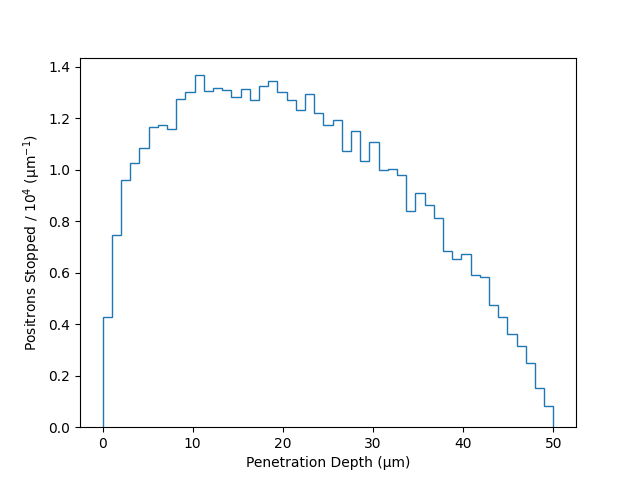
\includegraphics[width=\linewidth]{FoilModeratorStoppingDistance2.png}
          \caption{Before RF cavity}
          \label{fig:FoilStop2}
      \end{subfigure}
      \hfill
      \begin{subfigure}[b]{0.48\linewidth}
          \centering
          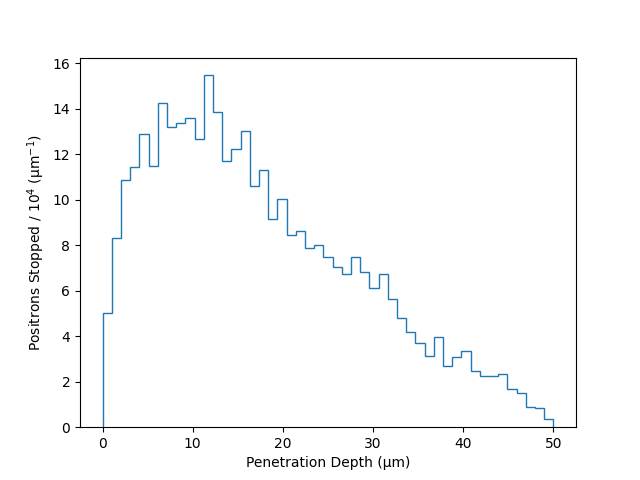
\includegraphics[width=\linewidth]{FoilModeratorStoppingDistance3.png}
          \caption{After RF cavity}
          \label{fig:FoilStop3}
      \end{subfigure}
      \caption{Stopping distributions of positrons at normal incidence, using the energy values from Fig.~\ref{fig:energytarget}.}
      \label{fig:FoilStopCombined}
  \end{figure}

Fig.~\ref{fig:FoilStop2} shows the stopping distribution the full energy spread generated in Fig.~\ref{fig:energytarget}. From Eq.~\ref{eq:therm}, we can calculate the expected positron yield $\gamma$,
\begin{equation}
    \gamma=\frac{1}{N}\sum_N P_\text{thermalization},
    \label{eq:posyield}
\end{equation}
where $N$ is the number of simulated particles. For the 50 µm foil, simulations show that $\gamma=1.49\pm0.55\times10^{-7}$. This represents the fraction of positrons produced by the target that thermalize and are reemitted by the moderator.

The overall efficiency of electrons converted to positrons was $3.81\pm1.41\times10^{-7}\text{ e}^+/\text{e}^-$. This compares to approximately $16\times10^{-7}\text{ e}^+/\text{e}^-$ for a positron source at LLNL~\cite{LLNLpositron} and $0.28\times10^{-7}\text{ e}^+/\text{e}^-$ for the GBAR experiment,~\cite{GBAR} though both setups differed from the design simulated here.


\section{Alternative Designs}
\subsection{Foil with AMD and RF Cavity}

High-energy positrons do not stop in the moderator, as shown in Fig.~\ref{fig:FoilEnergy}. Therefore, the decelerating RF cavity can increase the yield by lowering the beam energy. The new stopping distribution (Fig.~\ref{fig:FoilStop3}) has a yield of $\gamma=3.76\pm0.35\times10^{-6}$. This is approximately a 25.3x improvement over the case without the AMD and cavity. However, some positrons are lost during the intermediate stages, so the system efficiency is $6.2\pm0.57\times10^{-6}\text{ e}^+/\text{e}^-$, an improvement of 16.3x.


\subsection{Grid Moderator}
In addition to the foil, we simulate a mesh of foils based off of the moderator used at the Slow Positron Facility at KEK.~\cite{KEK} We use four planes of 25 µm foils along each axis (each separated by a 10 mm gap), surrounded by 7 mm of tungsten to act as the target (Fig.~\ref{fig:GridModerator}). This moderator had a yield of $\gamma=3.32\pm 0.26\times10^{-5}$, over twenty times greater than the foil moderator. However, the grid moderator comes at a cost of increased beam emittance, since the positrons are spread out over the entire moderator volume.

\begin{figure}
    \centering
    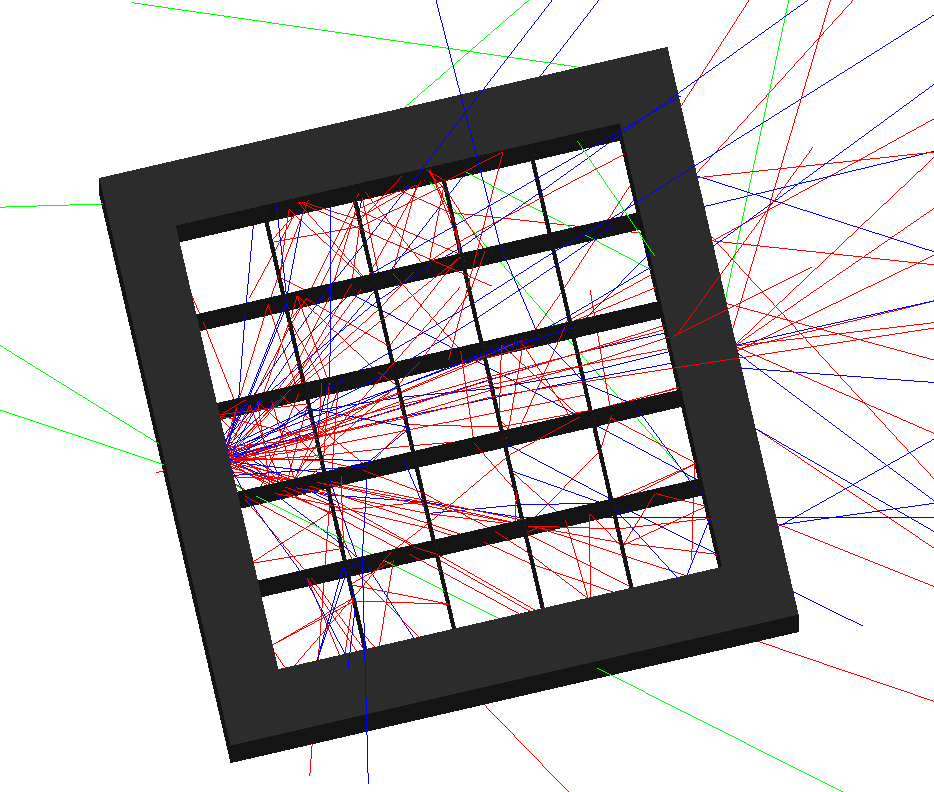
\includegraphics[width=\linewidth]{GridModeratorSchematic.png}
    \caption{Render of the moderator modeled off of the Slow Positron Facility at KEK. Electrons (red) hit the target from the leftmost edge and the resulting positrons (blue) stop in the mesh.}
    \label{fig:GridModerator}
\end{figure}

\subsection{Single-Crystal Moderator}
The final design tested was a single-crystal cylinder of tungsten. This has the advantage of a greater diffusion length, so a greater fraction of positrons at the surface are reemitted. However, this material cannot be a thin foil and is instead a block, meaning positrons can only emerge from one side of the moderator. The efficiency of this moderator was $\gamma=3.46\pm0.84\times10^{-6}$.

\section{Discussion}
\begin{figure}
    \centering
    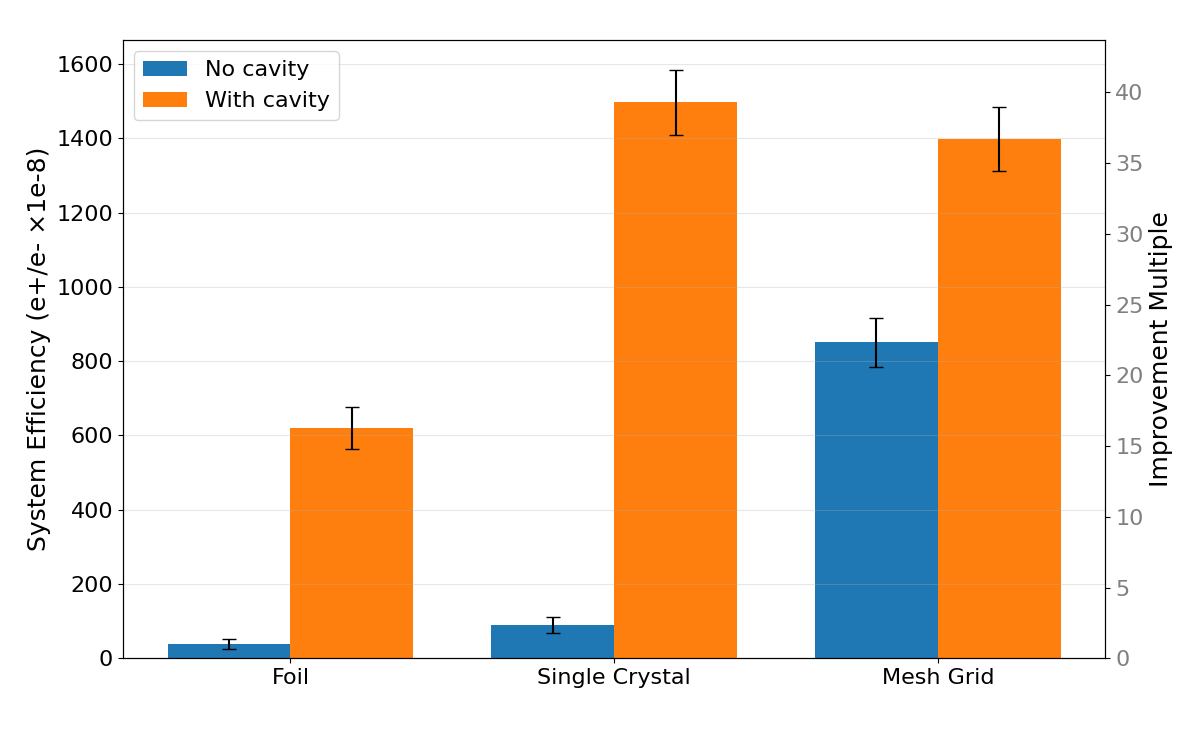
\includegraphics[width=\linewidth]{Summary.png}
    \caption{System efficiency of various moderator geometries, with and without the AMD and RF cavity. The right axis shows the improvement multiple in comparison to the foil moderator without a cavity.}
    \label{fig:Summary}
\end{figure}
The overall improvements to system efficiency is shown in Fig.~\ref{fig:Summary}. Adding the linac significantly improves efficiency to all geometry designs. In addition, we find that the single-crystal moderator is the best design for maximizing the yield of the positron source. With the linac, it has a 39.3x improvement over the traditional method of a simple polycrystalline foil moderator.

\section{Acknowledgements}
This work was supported by the Department of Energy, Laboratory Directed Research and Development program at SLAC National Accelerator Laboratory, under contract DE-AC02-76SF00515. This work was supported in part by the U.S. Department of Energy, Office of Science, Office of Workforce Development for Teachers and Scientists (WDTS) under the Science Undergraduate Laboratory Internships Program (SULI).

\bibliographystyle{aip}
\bibliography{paper}

\end{document}
